\subsection{Prof. Dr. Bettina Olk}


\textbf{Main Research Interests}\\[-0.25cm]
\begin{enumerate}
\item[$\bullet$]	Reflexive and Volitional Attention and their Dynamic Interaction
\item[$\bullet$]	Mechanisms of Saccadic Eye Movements and Target Selection
\item[$\bullet$]	Brain Mechanism Underlying Attention and Eye Movements
\item[$\bullet$]	Neuropsychological Syndromes: Spatial Neglect, Attention Disorders
\item[$\bullet$]	Special Populations: Attention in Autism Spectrum Disorders
\end{enumerate}


\vspace{0.6cm}
\textbf{Research Activities}\\[-0.25cm]

Orienting towards sources of information is a key prerequisite for an efficient interaction with our stimulus-rich environment. Reflexive orienting serves to guide attention very rapidly to areas of interest. Volitional orienting involves allocating attention in a goal-directed manner, e.g., based on the intention to attend to a specific stimulus. Depending on the stimuli and the task at hand, reflexive and volitional attention may be directed towards the same or opposing locations, the latter requiring the inhibition of reflexive orienting and the resolution of competition between reflexive and volitional factors. Bettina Olk's representative current projects investigate these kinds of orienting and how they interact, for example to control our eye movements. Many locations in our visual world potentially attract our attention and our gaze. But because we can only look at one point in space at a time, conflicts between candidate locations need be resolved. Current projects vary the demands on eye movement control and also aim at investigating the involvement of parietal and frontal cortex in such tasks by testing participants with brain injuries. Future studies (in collaboration with Prof. Hilgetag, IUB) will also apply Transcranial Magnetic Stimulation (TMS) to those brain areas to characterize their role. The research is conducted at IUB, at the University of Glasgow (with Dr. Monika Harvey) and the University of British Columbia (with Prof. Alan Kingstone). Further collaborations exist with several hospitals and rehabilitation centers in Bremen. A transdisciplinary research project (with Profs. Kappas and M�ller, IUB) investigates how different groups of people perceive press photography, how they interpret the visuals and how they react to them. The project is unique as it combines for the first time the methods of eye tracking (perception analysis), iconology (meaning interpretation) and psychophysiological measurement (emotional reaction).
\\
\begin{}
  \begin{center}
    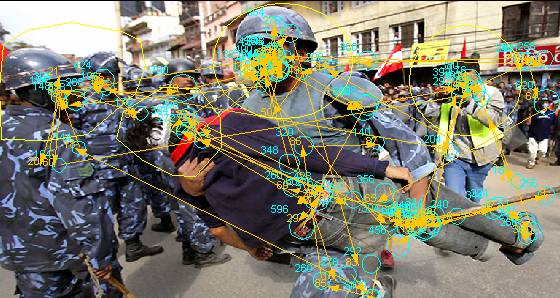
\includegraphics[width=0.8\textwidth]{./Psy/Olk.jpg}
    
    \caption{\itshape The picture shows a typical eye movement scanpath of a participant. Blue circles represent areas on which (and for how long) the participant fixated, yellow arrows illustrate eye movements.}%\label{fig:profxxx}
   \end{center}
\end{figure}


\newpage

\textbf{Funded Projects}\\[-0.25cm]
\begin{enumerate}
\item[$\bullet$]  "Integration of reflexive and volitional orienting: Comparing visual attention and eye movement control", in collaboration with Prof. Dr. Alan Kingstone, University of British Columbia, Canada, funded by the German Academic Exchange Service (DAAD)
\item[$\bullet$]  "Integration of reflexive and volitional orienting: Comparing motor systems", in collaboration with Dr. Monika Harvey, University of Glasgow, Scotland funded by The Royal Society
\end{enumerate}



\vspace{0.6cm}
\textbf{Other Professional Activities}\\[-0.25cm]
\begin{enumerate}
\item[$\bullet$] Reviewer for the following scientific journals: Experimental Brain Research, Journal of Experimental Psychology: Human Perception and Performance, Neuropsychologia, Perception, Perception \&
Psychophysics
\item[$\bullet$] Chair of the Academic Integrity Committee at IUB
\item[$\bullet$] Member of several international scientific organizations
\end{enumerate}


\vspace{0.6cm}
\textbf{Research Personnel}\\[-0.25cm]

Yu Jin\newline
Postdoctoral Fellow \\[-0.15cm]

